% SIAM Article Template
\documentclass[final,hidelinks,onefignum,onetabnum]{siamart220329}

% Information that is shared between the article and the supplement
% (title and author information, macros, packages, etc.) goes into
% ex_shared.tex. If there is no supplement, this file can be included
% directly.

% Packages and macros go here
\usepackage{lipsum}
\usepackage{amsfonts}
\usepackage{epstopdf}
\usepackage{url}
\usepackage{afterpage}
% \usepackage{algorithmic}
\ifpdf
  \DeclareGraphicsExtensions{.eps,.pdf,.png,.jpg}
\else
  \DeclareGraphicsExtensions{.eps}
\fi

%%%%%%%%%%%%%%%%%%%%%%%%%%%%%%%%%%%%%%%%%%%%%%%%%%%%%%%%%%%%%%%%%
% Paul's commands - note that some had to be commented out

\usepackage[normalem]{ulem}
\usepackage[labelfont=bf, size=small]{caption}
\usepackage[labelformat=empty, size=small]{subcaption}


\usepackage{microtype, fancyhdr,
  siunitx, graphicx, hyperref, epstopdf, tikz, adjustbox, mathtools, float,
  anyfontsize, relsize}
\usepackage{bm, amssymb, amsmath, mathrsfs}
\usepackage{etoolbox}
\usepackage[algo2e, ruled, linesnumbered, resetcount]{algorithm2e}
\SetFuncSty{textsc}
\SetKwProg{Function}{}{:}{}
\SetKwComment{Comment}{$\triangleright$\ }{}

\usepackage{enumitem}
\setlist[itemize]{leftmargin=2em, topsep=0.5\baselineskip, itemsep=0.5\baselineskip}


\newcommand{\I}{\mathcal{I}}   % Identity matrix
\newcommand{\E}{\mathbb{E}}    % Expectation
\newcommand{\V}{\mathbb{V}}    % Variance
\newcommand{\Z}{\mathbb{Z}}    % Integers
\newcommand{\Q}{\mathbb{Q}}    % Rational numbers
\newcommand{\R}{\mathbb{R}}    % Real numbers
\newcommand{\C}{\mathbb{C}}    % Complex numbers
\newcommand{\B}{\mathcal{B}}   % Borel set
\newcommand{\X}{\mathcal{X}}   % Italic X
\newcommand{\bO}{\mathcal{O}}  % "big O"
\newcommand{\Hs}{\mathcal{H}}  % Hilbert space
\newcommand{\Sc}{\mathcal{S}}  % Schwartz Class
\newcommand{\Fr}{\mathcal{F}}  % Fourier Transform operator
\newcommand{\Pw}{\mathcal{P}}  % Power set
\newcommand{\Nd}{\mathcal{N}}  % Normal distribution
\newcommand{\Pb}{\mathbb{P}}   % Probability set
\newcommand{\sv}{\, | \,}      % spaced vertical bar
\newcommand{\bt}{\beta}        % beta
\newcommand{\eps}{\varepsilon} % epsilon
\newcommand{\lam}{\lambda}     % lambda
\newcommand{\tht}{\theta}      % theta
\newcommand{\sgm}{\sigma}      % sigma
\newcommand{\omg}{\omega}      % omega
\newcommand{\gam}{\gamma}      % gamma
\newcommand{\bx}{\bm{x}}       % bold x
\newcommand{\by}{\bm{y}}       % bold y
\newcommand{\bv}{\bm{v}}       % bold v
\newcommand{\bu}{\bm{u}}       % bold u
\newcommand{\bz}{\bm{z}}       % bold z
\newcommand{\bw}{\bm{\omega}}  % bold omega
\newcommand{\bmu}{\bm{\mu}}    % bold mu
\newcommand{\bth}{\bm{\theta}} % bold theta
\newcommand{\bet}{\bm{\eta}}   % bold eta
\newcommand{\bS}{\bm{\Sigma}}  % bold Sigma
\newcommand{\bA}{\bm{A}}       % bold A
\newcommand{\syd}{\triangle}     % symmetric difference
\newcommand{\sem}{\setminus}     % set minus
\newcommand{\pluseq}{\ \mathsmaller{\mathrel{+}=}\ } % plus equals
\newcommand{\abs}[1]{\left|#1\right|}      % absolute value
\newcommand{\br}[1]{\overline{#1}}         % bar
\newcommand{\wht}[1]{\widehat{#1}}         % hat
\newcommand{\cvd}{\rightsquigarrow}        % convergence in distribution
\newcommand{\beps}{\bm{\eps}}              % bold epsilon
\newcommand{\pref}[1]{(\ref{#1})}          % ref in parentheses
\newcommand{\ind}[1]{\bm{1}_{\set{#1}}}    % Indicator function
\newcommand{\red}[1]{{\color{red} #1}}     % red text that is robust
\newcommand{\blue}[1]{{\color{blue} #1}}   % blue text that is robust
\newcommand{\dif}[1]{\mathop{}\!\mathrm{d}{#1}}   % d for dx in integral
% norm (\norm[p]{\bx} for p norm)
\newcommand{\norm}[2][]{\left\Vert#2\right\Vert_{#1}} % norm
\newcommand{\shortnorm}[2][]{\Vert#2\Vert_{#1}}       % short norm
\newcommand{\set}[1]{\left\{ #1\right\}}              % set notation
\newcommand{\flr}[1]{{\left\lfloor #1 \right\rfloor}} % floor function
\newcommand{\inp}[1]{\left\langle #1 \right\rangle}   % inner product
\newcommand{\mat}[1]{\begin{bmatrix}#1\end{bmatrix}}  % matrix
\newcommand{\tr}{\mathrm{tr}}
\renewcommand{\epsilon}{\varepsilon}

\DeclareMathOperator*{\Cov}{Cov} 
\DeclareMathOperator*{\Var}{Var}
\DeclareMathOperator*{\argmin}{arg\,min}   % argmin
\DeclareMathOperator*{\argmax}{arg\,max}   % argmax
\DeclareMathOperator*{\logdet}{logdet}     % logdet
\let\Re\relax \DeclareMathOperator*{\Re}{Re} 
\let\Im\relax \DeclareMathOperator*{\Im}{Im}
\newcommand{\range}[2]{#1\hspace*{-0.2em}:\hspace*{-0.2em}#2} % index range
\newcommand{\der}[2]{\frac{d #1}{d #2}} % derivative
\newcommand{\pder}[2]{\frac{\partial #1}{\partial #2}} % partial derivative
\newcommand{\iid}{\mathrel{\overset{\scalebox{0.5}{\text{i.i.d.}}}{\scalebox{1.1}[1]{$\sim$}}}}
% iid

\newtheorem{theorem}{Theorem}
\newtheorem*{theorem*}{Theorem}
\newtheorem{lemma}{Lemma}
\newtheorem*{lemma*}{Lemma}
\newtheorem{corollary}{Corollary}
\newtheorem*{corollary*}{Corollary}
\newtheorem{definition}{Definition}
\newtheorem*{definition*}{Definition}
\newtheorem{proposition}{Proposition}
\newtheorem*{proposition*}{Proposition}
\theoremstyle{remark}
\newtheorem{remark}{Remark}
\newtheorem*{remark*}{Remark}

\numberwithin{equation}{section}

\newcommand{\todocite}{\red{[CITE]}}

\newcommand{\Bloc}{B^{\textsc{\tiny \hspace*{-1pt} loc}}_{\nu,L}} 
\newcommand{\Basy}{B^{\textsc{\tiny \hspace*{-1pt} asy}}_{\nu,M}} 

\def\spacingset#1{\renewcommand{\baselinestretch}%
{#1}\small\normalsize} \spacingset{1}

\sisetup{exponent-mode=input, retain-zero-exponent=true}

%%%%%%%%%%%%%%%%%%%%%%%%%%%%%%%%%%%%%%%%%%%%%%%%%%%%%%%%%%%%%%%

% Add a serial/Oxford comma by default.
\newcommand{\creflastconjunction}{, and~}

% Used for creating new theorem and remark environments
\newsiamremark{remark}{Remark}
\newsiamremark{hypothesis}{Hypothesis}
\crefname{hypothesis}{Hypothesis}{Hypotheses}
\newsiamthm{claim}{Claim}

% Sets running headers as well as PDF title and authors
\headers{A Nonuniform Fast Hankel Transform}{Paul G. Beckman and Michael O'Neil}

% Title. If the supplement option is on, then "Supplementary Material"
% is automatically inserted before the title.
\title{A Nonuniform Fast Hankel Transform\thanks{Submitted to the editors DATE.
    \funding{P. G. Beckman was partially supported by the Office of Naval
      Research under award \#N00014-21-1-2383 and by the U.S.  Department of
      Energy, Office of Science, Office of Advanced Scientific Computing
      Research, Department of Energy Computational Science Graduate Fellowship
      under Award Number DE-SC0022158. M. O'Neil was partially supported by the
      Office of Naval Research under award \#N00014-21-1-2383.}  } }

% Authors: full names plus addresses.
\author{Paul G. Beckman\thanks{Courant Institute, New York University, New York, NY\\
  (\email{paul.beckman@cims.nyu.edu}, \url{https://cims.nyu.edu/\~pgb8409}).}
\and Michael O'Neil\thanks{Courant Institute, New York University, New York, NY\\
  (\email{oneil@cims.nyu.edu}, \url{https://cims.nyu.edu/\~oneil}).}
}

\usepackage{amsopn}
\DeclareMathOperator{\diag}{diag}

% Optional PDF information
\ifpdf
\hypersetup{
  pdftitle={A Nonuniform Fast  Hankel Transform}
  pdfauthor={P. G. Beckman and M. O'Neil}
}
\fi

% The next statement enables references to information in the
% supplement. See the xr-hyperref package for details.

%\externaldocument[][nocite]{ex_supplement}

% FundRef data to be entered by SIAM
%<funding-group specific-use="FundRef">
%<award-group>
%<funding-source>
%<named-content content-type="funder-name"> 
%</named-content> 
%<named-content content-type="funder-identifier"> 
%</named-content>
%</funding-source>
%<award-id> </award-id>
%</award-group>
%</funding-group>

\begin{document}

\maketitle

% REQUIRED
\begin{abstract}
  In this work we describe a fast algorithm for computing Hankel transforms of
moderate order which combine local and asymptotic expansions with nonuniform
Fast fourier transforms. The resulting algorithm executes in~$\bO (N
\log^2 N)$ time, where~$n$ denotes the number of points in both space and
frequency.  The algorithm can be executed to arbitrary precision, with the
length of the local and asymptotic expansions adjusted accordingly. Several
numerical examples are provided which demonstrate the speed of the algorithm in
multiple regimes, i.e. varying distributions of points and varying orders.

\end{abstract}

% REQUIRED
\begin{keywords}
Hankel transform, fast Fourier transform, asymptotic expansion, Bessel function
\end{keywords}

% REQUIRED
\begin{MSCcodes}
65R10, 33C10
\end{MSCcodes}

\section{Introduction} 

The fast Fourier transform (FFT) has revolutionized a wide range of applications
in mathematics, engineering, physics, etc., by enabling signal processing and
Fourier analysis tasks to be performed using a computational cost which scales
quasi-linearly with the number of data points~$n$. However, the FFT requires
that the input signal be sampled at equispaced points in time and that the
desired output frequencies are equispaced on the integers. These assumptions are
frequently not met in applications such as adaptive numerical PDE
solvers~\cite{alpert2002adaptive,jiang2023dual,askham2017adaptive,nochetto2009theory},
magnetic resonance
imaging~\cite{greengard2007fast,bondesson2019nonuniform,bronstein2002reconstruction},
and various signal processing
tasks~\cite{alexander2012adaptive,thakur2011synchrosqueezing}. To overcome this
setback, nonuniform FFT (NUFFT) algorithms have been
developed~\cite{dutt1993fast,greengard2004accelerating} which achieve near-FFT
speeds in one dimension, assuming that the distribution of time samples and
frequency outputs is not pathological. In higher dimensions, NUFFTs are less
competitive with standard FFTs, but the computational task at hand is also
significantly harder.

The FFT grew out of a need to perform Fourier transforms in Cartesian
coordinates. However, depending on the particular problem, the relevant
continuous Fourier analysis might be better suited to other coordinate systems.
One such commonly encountered situation is computing the Fourier transform of
radially symmetric functions in dimensions~$d \geq 2$. For example, in two
dimensions the Fourier transform of a function~$f$ is given by
\begin{equation}
  g(\omega_1, \omega_2) = \frac{1}{4\pi^2} \iint_{\R^2} f(x_1, x_2) \, 
  e^{-i(\omega_1 x_1 + \omega_2 x_2)}  \, dx_1 \, dx_2.
\end{equation}
Transforming to polar coordinates~$(\omega_1,\omega_2) \mapsto (\omega,\alpha)$
and~$(x_1,x_2) \mapsto (r,\theta)$ the above expression becomes
\begin{equation}
  \label{eq:ftpolar}
  \begin{aligned}
    g(\omega, \alpha) &= \frac{1}{4\pi^2} \int_0^{2\pi} \int_0^\infty
    f(r,\theta) \, 
    e^{-i \omega r (\cos\alpha \cos\theta + \sin\alpha \sin\theta) } 
    \, r \, dr \, d\theta \\
  &= \frac{1}{4\pi^2} \int_0^{2\pi} \int_0^\infty f(r,\theta) \, e^{-i \omega r \cos(\alpha-\theta) } \, r \, dr \, d\theta.
  \end{aligned}
\end{equation}
Furthermore, if~$f$ is radially symmetric, i.e.~$f(r, \theta) = f(r)$, then the
above transform can be written as
\begin{equation}
  \label{eq:HT}
  \begin{aligned}
  g(\omega,\alpha) &= \frac{1}{4\pi^2} \int_0^\infty f(r) \, r \int_0^{2\pi} 
  e^{-i \omega r \cos(\alpha - \theta) }  \, d\theta \, dr \\
  &= \frac{1}{2\pi} \int_0^\infty f(r) \, J_0(\omega r) \, r \, dr,
  \end{aligned}
\end{equation}
where we have used the integral representation of the zeroth-order Bessel
function~\cite{olver2010nist}
\begin{equation}
  J_0(x) 
  = \frac{1}{\pi} \int_0^\pi \cos \left( x \cos \theta \right) \, d\theta.
\end{equation}
The final integral involving~$J_0$ in equation~\eqref{eq:HT} is known as a
\emph{Hankel Transform} of order 0 --- usually referred to simply as a Hankel
Transform. 

In higher ambient dimensions, the Fourier transform of radially symmetric
functions reduces to a Hankel transform of higher order, which we treat toward
the end of this manuscript. Similarly, if the function~$f$ in~\eqref{eq:ftpolar}
has a particular periodic dependence in~$\theta$, e.g.~$f(r,\theta) =
f(r)e^{ik\theta}$, then we have
\begin{equation} \label{eq:FB-integral}
  \begin{aligned}
  g(\omega,\alpha) &= \frac{1}{4\pi^2} \int_0^\infty f(r) \, r \int_0^{2\pi} 
  e^{-i \omega r \cos(\alpha - \theta) } \, e^{ik\theta}  \, d\theta \, dr \\
  &= \frac{i^k}{2\pi} \int_0^\infty f(r) \, r \, J_k(\omega r)  \, dr,
  \end{aligned}
\end{equation}
where, again, we have invoked an integral representation
for~$J_k$~\cite{olver2010nist}. 

In order to numerically compute~$g$ in~\eqref{eq:HT} or~\eqref{eq:FB-integral}
at a collection of~$m$ ``frequencies''~$\omega_j$, the Hankel transform must be
discretized using an appropriate quadrature rule which depends on the particular
class of~$f$ for which the integral is desired. In general this results in the
need for computing
\begin{equation} \label{eq:DHT}
  \begin{aligned}
  g(\omega_j) \approx 
  g_j &:= \sum_{k=1}^n w_k \, f(r_k) \, r_k \, J_\nu(\omega_j r_k) \\
  &\ = \sum_{k=1}^n c_k \, J_\nu(\omega_j r_k)
   \qquad \text{for } j = 1, \ldots, m.
  \end{aligned}
\end{equation}
The above sum will be referred to as the Discrete Hankel Transform (DHT) of
order $\nu$. 

In our motivating example --- computing the continuous Fourier transform --- the
DHT arises from the discretization of the radially symmetric Fourier integral.
The DHT also appears in a wide range of applications including
imaging~\cite{higgins1988hankel, zhao2013fourier, marshall2023fast},
statistics~\cite{lord1954a, genton2002nonparametric}, and separation of
variables methods in partial differential
equations~\cite{bisseling1985fast,ali1999generalized, zhou2022spectral}. In many
such applications, a fully nonuniform DHT is desired, as the relevant
frequencies $\omega_j$ may not be equispaced, and the most efficient quadrature
rule for discretizing (\ref{eq:HT}) may have nodes $r_k$ which are also not
equispaced. It is enough to consider the above sum merely with the
coefficients~$c_k$. The algorithm of this work allows for arbitrary selection of
the frequencies~$\omega_j$ and nodes~$r_k$, in contrast to other algorithms
which require some structure to their location (e.g. equispaced). There are a
few types of commonly encountered DHTs, all of which our algorithm can address.
Schl\"omilch expansions~\cite{linton2006schlomilch,townsend2015fast}
take~$r_k \in [0,1]$ and the frequencies are chosen as~$\omega_j =
j\pi$. Fourier-Bessel expansions, often used in separation of variables
calculations for PDEs, take the frequencies~$\omega_j$ to be the ordered roots
of~$J_0$. In the most restrictive case, as discussed in~\cite{johnson1987improved}, the
frequencies~$\omega_j$ are set to be the ordered roots of~$J_\nu$, and the
nodes~$r_k$ a re set to be scaled roots of~$J_\nu$,
i.e.~$r_k = \mathrm{j}_{\nu,k}/\mathrm{j}_{\nu,k+1}$ where~$\mathrm{j}_{\nu,k}$
is the~$k$th largest root of~$J_\nu$ (which doesn't explicitly appear in the sum
above). Analogues of all these special cases exist when~$J_0$ is replaced with a
higher order bessel function~$J_m$ as well, but we do not go into the details as
our algorithm handles them all similarly.

\subsection*{Existing methods}
\label{sec:existing}

A number of methods exist in the literature to evaluate (\ref{eq:HT}) and
(\ref{eq:DHT}). These include series expansion methods
\cite{lord1954b,brunol1977fourier,cavanagh1979numerical}, convolutional
approaches \cite{siegman1977quasi, johansen1979fast, mook1983algorithm}, and
projection-slice or Abel transform-based methods \cite{oppenheim1980computation,
hansen1985fast, kapur1995algorithm}. See~\cite{cree1993algorithms} for a review
of many of these early computational approaches. Unfortunately, these existing
methods are either not applicable to the discrete case, require a particular
choice of $\omega_j$ or $r_k$ due to the constraints of interpolation or
quadrature subroutines, or suffer from low accuracy as a result of intermediate
approximations. Therefore, extending these schemes to compute the fully
nonuniform DHT with controllable accuracy is not straightforward.

A notable contribution is~\cite{liu1999nonuniform}, which describes a fully
nonuniform fast Hankel transform, although it has accuracy and speed
limitations. This work takes the popular convolutional approach, using a change
of variables to reformulate the Hankel transform as a convolution with a known
kernel. However, its accuracy is limited by the need for a quadrature on the
nonuniform points $r_k$ in order to compute the continuous Fourier transform.
The authors use an irregular trapezoidal rule for this purpose, which is not
high-order accurate. This method also requires the computation of the inverse
NUFFT using conjugate gradients. For even moderately clustered points or
frequencies, this inverse problem is extremely ill-conditioned, and thus the
number of required iterations can be prohibitive. This method is therefore
suitable for ``quasi-equispaced'' points and frequencies, but is not tractable
for all distributions.

More recently, butterfly algorithms \cite{oneil2010algorithm, li2015butterfly,
pang2020interpolative} were introduced as a broadly applicable methodology for
rapidly computing oscillatory transforms including the nonuniform DHT. However,
these algorithms require a precomputation or factorization stage for each new
set of $\omega_j$ and $r_k$. Such precomputations can, unfortunately, be a
bottleneck for applications in which these evaluation points change with each
iteration or application of the transform. In order to provide a
precomputation-free fast DHT,~\cite{townsend2015fast} employs a combination of
asymptotic expansions and Bessel function identities evaluated using the
equispaced FFT. The resulting scheme is applicable to equispaced or perturbed
``quasi-equispaced'' grids, for example $j_{0,k} / j_{0,n+1}$ where $j_{\nu,k}$
is the $k^{th}$ zero of $J_\nu$.

\subsection*{Novelty of this work}
\label{sec:novelty}

% At a high level, our algorithm can be viewed as a generalization of the one
% described in~\cite{townsend2015fast}. In~\cite{townsend2015fast}, asymptotic
% expansions were used to replace~$J_0$ for various arguments. These asymptotic
% expansions involved trigonometic functions, resulting in a fast algorithm for
% computing the DHT using fast cosine transforms (FCTs) and fast sine transforms
% (FSTs). In order to invoke these fast algorithms, various assumptions
% on~$\omega_j$ and~$r_k$ had to be made.

We describe here a precomputation-free nonuniform fast Hankel transform (NUFHT)
which generalizes~\cite{townsend2015fast} to the fully nonuniform setting in a
number of ways. First, we employ an adaptive partitioning scheme which, for any
choice of $\omega_j$ and $r_k$, subdivides the matrix with
entries~$J_\nu(\omega_j r_k)$ into blocks for which matrix-vector products can
be evaluated efficiently. Second, we use the nonuniform fast Fourier transform
(NUFFT) to evaluate asymptotic expansions for nonuniform $r_k$ and $\omega_j$.
Finally, we utilize the low-rank expansion of $J_\nu$ given
in~\cite{wimp1962polynomial} in the local regime where asymptotic expansions are
not applicable. We derive error bounds for this low-rank expansion, allowing us
to choose all approximation parameters automatically by analysis which
guarantees that the resulting error is bounded by the user-specified tolerance
$\epsilon$.

\subsection*{Outline of the paper}

The paper is organized as follows. In Section~\ref{sec:overview} we give a high
level view of our algorithm, omitting technical details. Then in
Section~\ref{sec:approx} we study the local and asymptotic expansions of Bessel
functions which serve as the key building blocks of the algorithm. Afterward, in
Section~\ref{sec:methods}, we provide a detailed description of the algorithm
and its associated complexity. Various numerical examples are provided in
Section~\ref{sec:results}, and we conclude with some additional discussion in
Section~\ref{sec:discussion}.




%%% Local Variables:
%%% mode: latex
%%% TeX-master: "../main"
%%% End:


\section{Overview of the algorithm} \label{sec:overview}

To more concisely describe our approach, we write the DHT (\ref{eq:DHT}) as the
equivalent matrix-vector product with $\mtx{A} \in \R^{m \times n}$
\begin{equation}
    \vct{g} = \mtx{A}\vct{f}, \qquad \mtx{A}(j,k) = J_\nu(\omega_j r_k).
\end{equation}
The matrix $\mtx{A}$ is in general full rank and possesses complex oscillatory
structure. As a result, no straightforward fast algorithm exists to apply the
full matrix $\mtx{A}$ to a vector. However, we devise an NUFHT by noting that
certain \textit{blocks} $\mtx{A}(j_0:j_1, k_0:k_1)$ are able to be applied to a
vector rapidly using analytical expansions of the underlying Bessel function
$J_\nu$. 

When the argument $\omega_j r_k$ is small, $J_\nu$ is smooth and essentially
non-oscillatory, and we use a closed-form local expansion which approximates
$J_\nu$ in terms of Chebyshev polynomials, yielding a low-rank approximation to
the block $\mtx{A}(j_0:j_1, k_0:k_1)$ that can be applied to a vector in linear
time. When the argument $\omega_j r_k$ is large, we use a classical asymptotic
expansion which expresses $J_\nu$ as a sum of a small number of decaying
sinusoids, and can therefore be applied to a vector in quasilinear time using
the NUFFT. Figure~\ref{fig:two-expansions} shows the oscillatory behavior of
$J_0$, as well as the accuracy of these local and asymptotic expansions.

By analyzing the error in these two expansions, we can choose a threshold $z$
such that an $L$-term local expansion and an $M$-term asymptotic expansion are
both guaranteed to be accurate to the desired tolerance $\epsilon$ in the
regions $\omega_j r_k \leq z$ and $\omega_j r_k > z$ respectively. Next, we
adaptively subdivide $\mtx{A}$ into disjoint blocks so that either $\omega_j r_k
\leq z$ or $\omega_j r_k > z$ for all $\omega_j$ and all $r_k$ in each block.
This leaves only a few small blocks with $\omega_j r_k \approx z$ whose entries
can be directly computed. Finally, we apply each of these disjoint blocks of
$\mtx{A}$ to $\vct{f}$ using the corresponding fast method.
Figure~\ref{fig:subdivide} shows an Hankel transform matrix $\mtx{A}$ divided
into local and asymptotic entries along the curve $\omega r = z$, as well as the
corresponding adaptive subdivision of the matrix into blocks which can be
rapidly applied.

\begin{figure}
  \centering
  \begin{subfigure}[b]{0.45\textwidth}
    \includegraphics[width=\textwidth]{./figures/bessel_function.pdf}
  \end{subfigure}
  \begin{subfigure}[b]{0.45\textwidth}
    \includegraphics[width=\textwidth]{./figures/pointwise_errors.pdf}
  \end{subfigure}
  \caption{Bessel function $J_0(z)$ and pointwise relative error in
  approximating $J_0(z)$ using local and asymptotic expansions. Dotted vertical
  line shows crossover point where both expansions are accurate to $\epsilon =
  10^{-12}$.}
  \label{fig:two-expansions}
\end{figure}

\begin{figure}
  \centering
  \newcommand\twa{0.29cm} \newcommand\tw{0.43cm}
  \begin{subfigure}[b]{0.28\textwidth}
    \begin{tikzpicture}
        \draw (0, 0) node[inner sep=0] {\includegraphics[width=0.75\textwidth,
        trim={\twa, \twa, \twa, \twa}, clip]{./figures/splitting.pdf}}; \draw
        (-0.8, 0.8) node {\small \textbf{Local}}; \draw (0.3, -0.7) node {\small
        \textbf{Asymptotic}}; \draw (0, 1.6) node {\small $r_1 \ \; < \ \dots \
        < \ \; r_n$}; \draw (-1.7, 0) node[align=center] {\small $\omega_1$
        \\[3pt] $\wedge$ \\[3pt] $\vdots$ \\[3pt] $\wedge$ \\[3pt] $\omega_m$};
    \end{tikzpicture}
    \caption{}
  \end{subfigure}
  \hspace*{0.0\textwidth}
  \begin{subfigure}[b]{0.21\textwidth}
    \includegraphics[width=\textwidth, trim={\tw, \tw, \tw, \tw}, clip]{./figures/splitting_lvl1.pdf}
    \caption{Level 1}
  \end{subfigure}
  \hfill
  \begin{subfigure}[b]{0.21\textwidth}
    \includegraphics[width=\textwidth, trim={\tw, \tw, \tw, \tw}, clip]{./figures/splitting_lvl2.pdf}
    \caption{Level 2}
  \end{subfigure}
  \hfill
  \begin{subfigure}[b]{0.21\textwidth}
    \includegraphics[width=\textwidth, trim={\tw, \tw, \tw, \tw}, clip]{./figures/splitting_lvl3.pdf}
    \caption{Level 3}
  \end{subfigure}
  \caption{Splitting of Hankel transform matrix $\mtx{A}$ along the curve
  $\omega r = z$ into local and asymptotic regions. Adaptive subdivision of
  $\mtx{A}$ into corresponding local (red), asymptotic (blue), and mixed (gray)
  sub-blocks at various levels.}
  \label{fig:subdivide}
\end{figure}

\section{Bessel function approximations} \label{sec:approx}
We now describe local and asymptotic expansions of the Bessel function
$J_\nu(\omega r)$, and provide error analysis by which one can select the number
of terms needed in each expansion to assure $\epsilon$ accuracy in both regimes.

\subsection{The Wimp expansion}\label{sec:local}

Near the origin, $J_\nu(z)$ is a smooth and essentially non-oscillatory function
of $z$. As a result, $J_\nu(xy)$ is a numerically low-rank function of all
sufficiently small inputs $x$ and $y$. Fortuitously, one such low-rank expansion
--- which we refer to as the \textit{Wimp expansion} --- is available in closed
form for integer~$\nu$~\cite{wimp1962polynomial}. In the case that $\nu$ is
even, we have
\begin{equation}
    \begin{aligned}
        J_\nu(xy) 
        &= \sum_{\ell=0}^\infty C_\ell(x) \, T_{2\ell}(y) \\
        C_\ell(x) 
        &= \delta_\ell \, J_{\frac{\nu}{2} + \ell}(x) \, J_{\frac{\nu}{2} - \ell}(x) \\
        \delta_\ell 
        &= \begin{cases}
            1 & \ell=0 \\
            2 & \text{otherwise}
        \end{cases}
    \end{aligned}
\end{equation}
for all $\abs{y} \leq 1$. A similar expansion exists for $\nu$ odd.

In order to employ the Wimp expansion to compute local terms within the Hankel
transform, we must determine the number of terms $L$ needed to construct an
$\epsilon$-accurate approximation to $J_\nu(\omega r)$ on a given rectangle
$(\omega, r) \in [0, \Omega] \times [0, R]$. The following lemma provides a
bound on the induced truncation error in the Wimp expansion as a function of the
order $\nu$, the space-frequency product $\Omega R$, and the number of retained
terms $L$.

\begin{lemma} \label{lem:wimp} Truncating the Wimp expansion after $L$ terms
    gives
    \begin{align}
        \abs{J_\nu(\omega r) - \sum_{\ell=0}^L C_\ell(\omega R) T_{2\ell}\left( \frac{r}{R} \right)} 
        \leq \frac{2\exp\left\{ \frac{\nu}{2}(\beta - \gamma) + (L+1)(\beta + \gamma) \right\}}{1 - e^{\beta + \gamma}}
    \end{align}
    for all $\omega \in [0, \Omega], r \in [0, R]$, where
    \begin{align}
        \psi(p) &:= \log p + \sqrt{1 - p^2} - \log\left( 1 + \sqrt{1 - p^2} \right) \\
        \beta &:= \psi\left( \frac{\Omega R}{2L + 2 + \nu} \right) \\
        \gamma &:= \begin{cases}
            \psi\left( \frac{\Omega R}{2L + 2 - \nu} \right) & L + 1 \geq \frac{\nu}{2} \\
            0 & \textnormal{otherwise}
        \end{cases}
    \end{align}
\end{lemma}
\begin{proof}
    For $\nu$ even, the truncation error after $L$ terms is bounded by
    \begin{align}
        \abs{\sum_{\ell=L+1}^\infty C_\ell(\omega R) T_{2\ell}\left( \frac{r}{R} \right)}
        &\leq 2\sum_{\ell=L+1}^\infty \abs{J_{\frac{\nu}{2} + \ell}\left(\frac{\omega R}{2}\right)} \abs{J_{\frac{\nu}{2} - \ell}\left(\frac{\omega R}{2}\right)}.
    \end{align}
    Define $p_\ell(\omega) := \omega R / (\nu + 2\ell)$. Then by Siegel's bound
    \cite[10.14.5]{olver2010nist} we have
    \begin{align}
        \abs{J_{\frac{\nu}{2} + \ell}\left(\frac{\omega R}{2}\right)}
        &= \abs{J_{\frac{\nu}{2} + \ell}\bigg(\Big(\frac{\nu}{2} + \ell\Big) p_\ell(\omega)\bigg)} \\
        &\leq \exp\left\{ \Big(\frac{\nu}{2} + \ell\Big) \psi\big(p_\ell(\omega)\big)\right\} \\
        &\leq \exp\left\{ \Big(\frac{\nu}{2} + \ell\Big) \beta \right\},
    \end{align}
    where the last inequality follows from the fact that $\psi$ is an increasing
    function on $(0,1)$, and thus $\psi\big(p_\ell(\omega)\big) \leq \beta < 0$
    for all $\ell \geq L+1$ and all $\omega \in [0, \Omega]$. 
    
    If $L+1 \geq \frac{\nu}{2}$, we define $q_\ell(\omega) := \omega R / (2\ell
    - \nu)$ and apply Siegel's bound again to obtain
    \begin{align}
        \abs{J_{\frac{\nu}{2} - \ell}\left(\frac{\omega R}{2}\right)}
        &= \abs{J_{\ell - \frac{\nu}{2}}\bigg(\Big(\ell - \frac{\nu}{2}\Big) q_\ell(\omega)\bigg)} 
        \leq \exp\left\{ \Big(\ell - \frac{\nu}{2}\Big) \gamma \right\}.
    \end{align}
    If $L+1 < \frac{\nu}{2}$, Siegel's bound does not apply and we use instead
    the simple bound $\abs{J_{\frac{\nu}{2} - \ell}\left(\frac{\omega
    R}{2}\right)} \leq 1$, which is equivalent to taking $\gamma = 0$. 

    All that remains is to apply a geometric series argument
    \begin{align}
        \abs{J_\nu(\omega r) - \sum_{\ell=0}^L C_\ell(\omega R) T_{2\ell}\left( \frac{r}{R} \right)}
        &\leq 2\sum_{\ell=L+1}^\infty \exp\left\{ \Big(\frac{\nu}{2} + \ell\Big) \beta + \Big(\ell - \frac{\nu}{2}\Big) \gamma \right\} \\
        &= 2\exp\left\{\frac{\nu}{2}(\beta - \gamma)\right\} \sum_{\ell=L+1}^\infty \left( e^{\beta + \gamma} \right)^\ell \\
        &= \frac{2\exp\left\{ \frac{\nu}{2}(\beta - \gamma) + (L+1)(\beta + \gamma) \right\}}{1 - e^{\beta + \gamma}}
    \end{align}
    A similar calculation can be carried out for $\nu$ odd.
\end{proof}

Lemma \ref{lem:wimp} is rather opaque regarding the impact of the various
parameters on the error because we have not utilized any simplifying bounds on
the function $\psi$. However, it takes into account the decay in both
$J_{\frac{\nu}{2}+\ell}$ \textit{and} $J_{\frac{\nu}{2}-\ell}$, thus remaining
relatively tight for small $\nu$. It is therefore well-suited to our purposes
because given $z, L > 0$, it gives a bound on the pointwise error in
approximating any block of the matrix $J_\nu(\omega_j r_k)$ for which $\omega r
\leq z$ using the $L$-term Wimp expansion. 

This expansion is highly beneficial from a computational perspective, as it
yields an analytical rank-$L$ approximation to any block of $\bm{A}$ for which
$\omega_j r_k$ is sufficiently small
\begin{equation}
  \mtx{A}(j_0:j_1, k_0:k_1)
  %\vct{f}(k_0:k_1)
  \approx \mtx{C}\mtx{T}^\top
  %\vct{f}(k_0:k_1)
\end{equation}
where $\mtx{C} \in \R^{(j_1-j_0+1) \times L}$ and $\mtx{T} \in \R^{(k_1-k_0+1)
  \times L}$ with entries
\begin{equation}
  \mtx{C}(j,\ell) = C_{\ell-1}(\omega_j r_{k_1}) \qquad  \text{and} \qquad 
  \mtx{T}(k,\ell) = T_{2\ell-2}\left(\frac{r_k}{r_{k_1}}\right).
\end{equation}
For a block of
$\mtx{A}$ of size $m_b \times n_b$, the low-rank approximation given by the Wimp
expansion can be applied to a vector in $\bO\big(L(m_b + n_b)\big)$ time by
first applying $\bm{T}^\top$ then applying $\bm{C}$.

\subsection{Hankel's expansion}
\label{sec:asymptotic}

Away from the origin, $J_\nu(z)$ exhibits essentially sinusoidal oscillation
with period $2\pi$. This statement is made precise by Hankel's asymptotic
expansion, which states that for $z \to \infty$
\begin{align} \label{eq:asymptotic-expansion}
    J_\nu(x)
    \sim \sqrt{\frac{2}{\pi x}} \left( 
        \cos\left(x + \phi\right) \sum_{\ell=0}^{\infty} \frac{(-1)^\ell a_{2\ell}(\nu)}{x^{2\ell}}
        - \sin\left(x + \phi\right) \sum_{\ell=0}^{\infty} \frac{(-1)^\ell a_{2\ell+1}(\nu)}{x^{2\ell+1}}
        \right)
\end{align}
where $\phi := - \frac{(2\nu+1)\pi}{4}$ and 
\begin{align}
    a_\ell(\nu) := \frac{(4\nu^2 - 1)(4\nu^2 - 3)\dots(4\nu^2 -
  (2\ell-1)^2)}{\ell! \, 8^\ell}.
\end{align}
Rearranging this expansion, we obtain an expansion which can be evaluated using
two NUFFTs and diagonal scalings, and whose error is bounded by the size of the
first neglected terms \todocite
\begin{multline}
     \Bigg| J_\nu(\omega r)
    - \sqrt{\frac{2}{\pi}} \sum_{\ell=0}^{M-1} \left[  
        \frac{(-1)^\ell a_{2\ell}(\nu)}{\omega^{2\ell + \frac{1}{2}}} \Re\left(
          \frac{e^{i\phi}}{r^{2\ell+\frac{1}{2}}} e^{i\omega r}\right) \right.
        \\ \left. - \frac{(-1)^\ell
            a_{2\ell+1}(\nu)}{\omega^{2\ell+\frac{3}{2}}}
          \Im\left(\frac{e^{i\phi}}{r^{2\ell+\frac{3}{2}}} e^{i\omega r} \right) \right]
        \Bigg| 
         \leq \sqrt{\frac{2}{\pi}} \left( \frac{\abs{a_{2M}(\nu)}}{(\omega r)^{2M+\frac{1}{2}}} + \frac{\abs{a_{2M+1}(\nu)}}{(\omega r)^{2M+\frac{3}{2}}} \right)
\end{multline}

The computational advantage of this expansion is that the $2M$-term asymptotic
expansion of any block of $\bm{A}$ can be rapidly applied to a vector~$\vct{x}$ using $2M$
Type-III NUFFTs
\begin{multline}
    \mtx{A}(j_0:j_1, k_0:k_1) \vct{x} 
    \approx \sqrt{\frac{2}{\pi}} \sum_{\ell=0}^{M-1} (-1)^\ell \Bigg[ 
        a_{2\ell}(\nu) \mtx{D}_\omega^{-2\ell-\frac{1}{2}} \Re\Big(e^{i\phi}
                                                             \mtx{F}
                                                             \mtx{D}_r^{-2\ell-\frac{1}{2}}
                                                             \vct{x} \Big) \\
        - a_{2\ell+1}(\nu) \mtx{D}_\omega^{-2\ell-\frac{3}{2}}
                                                             \Im\Big(e^{i\phi}
                                                               \mtx{F}
                                                               \mtx{D}_r^{-2\ell-\frac{3}{2}}
                                                               \vct{x} \Big) 
    \Bigg]
\end{multline}
where $\mtx{F} \in \C^{(j_1 - j_0 + 1) \times (k_1 - k_0 + 1)}$ is the Type-III
nonuniform DFT matrix corresponding to frequencies $\omega_{j_0}, \dots,
\omega_{j_1}$ and points $r_{k_0}, \dots, r_{k_1}$, and the diagonal scaling
matrices are given by $\mtx{D}_\omega :=
\diag(\omega_{j_0},\dots,\omega_{j_1})$, and $\mtx{D}_r :=
\diag(r_{k_0},\dots,r_{k_1})$.





\subsection{Determining order of expansions and crossover point}
\label{sec:cutoff}

With these error bounds in hand, we can precompute the
parameters~$z_{\nu, \epsilon}^M$ and~$L_{\nu, \epsilon}^M$ for tolerances
$\epsilon = 10^{-4}, \dots, \allowbreak 10^{-15}$, orders $\nu = 1, \dots, 100$,
and number of asymptotic expansion terms $M = 1, \dots, 20$:
\begin{itemize}
    \item $z_{\nu, \epsilon}^M$ such that $M$-term Hankel expansion of
    $J_\nu(\omega r)$ is $\epsilon$-accurate $\forall \ \omega r > z_{\nu,
    \epsilon}^M$,
    \item $L_{\nu, \epsilon}^M$ such that $L_{\nu, \epsilon}^M$-term Wimp
    expansion of $J_\nu(\omega r)$ is $\epsilon$-accurate $\forall \ \omega r
    \leq z_{\nu, \epsilon}^M$.
\end{itemize}
Therefore, for any order $\nu$ we can look up a pair of complementary local and
asymptotic expansions with error everywhere bounded by the requested tolerance
$\epsilon$. The only remaining free parameter is the number of asymptotic terms
$M$. This parameter is selected based on various numerical experiments which
maximize speed by balancing the cost of the local, asymptotic, and direct
evaluations. In our implementation, we use the heuristic
\begin{equation}
  \label{eq:num-asy-terms}
    M = \min\left(\flr{1 + \frac{\nu}{5} - \frac{\log_{10}(\epsilon)}{4}}, 20\right).
\end{equation}




%%% Local Variables:
%% mode: latex
%% TeX-master: "../main"
%% End:


\section{The Nonuniform Fast Hankel Transform} \label{sec:methods}

\subsection{Asymptotic expansion}

Hankel's expansion for $\omega r \to \infty$ is
\begin{equation}
    J_\nu(\omega r)
    \sim \sqrt{\frac{2}{\pi\omega r}} \left( 
        \cos\left(\mu\right) \sum_{\ell=0}^\infty (-1)^\ell \frac{a_{2\ell}(\nu)}{(\omega r)^{2\ell}}
        - \sin\left(\mu\right) \sum_{\ell=0}^\infty (-1)^\ell \frac{a_{2\ell+1}(\nu)}{(\omega r)^{2\ell+1}}
        \right)
\end{equation}
where $\mu := \omega r - \frac{(2\nu+1)\pi}{4}$ and 
\begin{equation}
    a_p(\nu) := \frac{(4\nu^2 - 1)(4\nu^2 - 3)\dots(4\nu^2 - (2p-1)^2)}{p! 8^p}.
\end{equation}
This expansion provides a means of evaluating products 

Hankel's expansion and evaluation with the NUFFT

Error bound

\subsection{Local expansion}

Wimp expansion and evaluation as low-rank matrix block

\begin{lemma} \label{lem:wimp} Truncating the Wimp expansion after $K$ terms
    gives
    \begin{equation}
        \abs{J_\nu(\omega r) - \sum_{k=0}^K C_{2k}(\omega R) T_{2k}\left( \frac{r}{R} \right)} 
        \leq \frac{2\exp\left\{ \frac{\nu}{2}(\beta - \gamma) + (K+1)(\beta + \gamma) \right\}}{1 - e^{\beta + \gamma}}
    \end{equation}
    for all $\omega \in [0, \Omega], r \in [0, R]$, where
    \begin{align}
        \psi(p) &:= \log p + \sqrt{1 - p^2} - \log\left( 1 + \sqrt{1 - p^2} \right) \\
        \beta &:= \psi\left( \frac{\omega R}{\nu + 2K + 2} \right) \\
        \gamma &:= \begin{cases}
            \psi\left( \frac{\omega R}{2K + 2 - \nu} \right) & K + 1 \geq \frac{\nu}{2} \\
            0 & \text{otherwise}
        \end{cases}
    \end{align}
\end{lemma}
\begin{proof}
    For $\nu$ even, the truncation error after $K$ terms is bounded by
    \begin{align}
        \abs{\sum_{k=K+1}^\infty C_{2k}(\omega R) T_{2k}\left( \frac{r}{R} \right)}
        &\leq 2\sum_{k=K+1}^\infty \abs{J_{\frac{\nu}{2} + k}\left(\frac{\omega R}{2}\right)} \abs{J_{\frac{\nu}{2} - k}\left(\frac{\omega R}{2}\right)}.
    \end{align}
    Define $p_k := \omega R / (\nu + 2k)$. Then by Siegel's bound
    \cite[10.14.5]{olver2010nist} we have
    \begin{align}
        \abs{J_{\frac{\nu}{2} + k}\left(\frac{\omega R}{2}\right)}
        &= \abs{J_{\frac{\nu}{2} + k}\bigg(\Big(\frac{\nu}{2} + k\Big) p_k\bigg)}
        \leq \exp\left\{ \Big(\frac{\nu}{2} + k\Big) \beta \right\},
    \end{align}
    where the last inequality follows from the fact that $\psi$ is an increasing
    function on $(0,1]$, and thus $\psi\left(p_k\right) \leq \beta < 0$
    for all $k \geq K+1$. 
    
    If $K+1 \geq \frac{\nu}{2}$, we define $q_k := x / (2k -
    \nu)$ and apply Siegel's bound again to obtain
    \begin{align}
        \abs{J_{\frac{\nu}{2} - k}\left(\frac{\omega R}{2}\right)}
        &= \abs{J_{k - \frac{\nu}{2}}\bigg(\Big(k - \frac{\nu}{2}\Big) q_k\bigg)} 
        \leq \exp\left\{ \Big(k - \frac{\nu}{2}\Big) \gamma \right\}.
    \end{align}
    If $K+1 < \frac{\nu}{2}$, Siegel's bound does not apply and we use instead
    the simple bound $\abs{J_{\frac{\nu}{2} - k}\left(\frac{\omega R}{2}\right)}
    \leq 1$, which is equivalent to taking $\gamma = 0$. 

    All that remains is to apply a geometric series argument
    \begin{align}
        \abs{J_\nu(\omega r) - \sum_{k=0}^K C_{2k}(\omega R) T_{2k}\left( \frac{r}{R} \right)}
        &\leq 2\sum_{k=K+1}^\infty \exp\left\{ \Big(\frac{\nu}{2} + k\Big) \beta + \Big(k - \frac{\nu}{2}\Big) \gamma \right\} \\
        &= 2\exp\left\{\frac{\nu}{2}(\beta - \gamma)\right\} \sum_{k=K+1}^\infty \left( e^{\beta + \gamma} \right)^k \\
        &= \frac{2\exp\left\{ \frac{\nu}{2}(\beta - \gamma) + (K+1)(\beta + \gamma) \right\}}{1 - e^{\beta + \gamma}}
    \end{align}
    A similar calculation can be carried out for $\nu$ odd.
\end{proof}

This result is rather opaque regarding the impact of the various parameters
because we have not utilized any bounds to simplify the function $\psi$.
However, it remains relatively tight for $\nu = 0$ and is sufficient for our
purposes, because given $z, K > 0$, Lemma \ref{lem:wimp} gives a bound on the
pointwise error in approximating any block of the matrix $J_\nu(\omega_j r_k)$
for which $\omega r \leq z$ using the $K$-term Wimp expansion. 

\subsection{Determining the cutoff between expansions}

With these error bounds in hand, we precompute the following tables for
tolerances $\epsilon = \texttt{1e-4}, \dots, \texttt{1e-15}$, orders $\nu = 1,
\dots, 20$, and number of asymptotic expansion terms $M = 1, \dots, 20$
\begin{itemize}
    \item $z_{\nu, \epsilon}^M$ such that the $M$-term asymptotic expansion of
    $J_\nu(\omega r)$ is $\epsilon$-accurate for all $\omega r > z_{\nu,
    \epsilon}^M$
    \item $K_{\nu, \epsilon}^M$ such that the $K_{\nu, \epsilon}^M$-term Wimp
    expansion of $J_\nu(\omega r)$ is $\epsilon$-accurate for all $\omega r \leq
    z_{\nu, \epsilon}^M$
\end{itemize}
Therefore, for any order $\nu$ we can look up a pair of complementary local and
asymptotic expansions with error everywhere bounded by the requested tolerance
$\epsilon$. The only remaining free parameter is the number of asymptotic terms
$M$. This parameter is selected heuristically in our implementation as 
\begin{equation}
    M = \min\left(\flr{1 + \frac{\nu}{5} - \frac{\log_{10}(\epsilon)}{4}}, 20\right)
\end{equation}
according to numerical experiments which maximize speed by balancing the cost of
the local, asymptotic, and direct evaluations.

\subsection{Subdividing the matrix into blocks by expansion}

Having established error bounds which allow us to automatically select the
number of asymptotic terms $M$, local terms $K$, and crossover point $z$ given a
tolerance $\epsilon$ and order $\nu$, we now discuss how to subdivide the matrix
$\bm{A}$ into three sets of blocks, each of which can be efficiently evaluated
as described above
\begin{itemize}
    \item Asymptotic blocks $\mathscr{A} = \big\{ (J, K) : \omega_j r_k > z \
    \forall \ j \in J, \ k \in K \big\}$
    \item Local blocks $\mathscr{L} = \big\{ (J, K) : \omega_j r_k \leq z \
    \forall \ j \in J, \ k \in K \big\}$
    \item Direct blocks $\mathscr{D}$ which are small enough that no fast
    expansion is needed
\end{itemize}
The idea is to consider index pairs $(j,k)$ such that $\omega_j r_k \approx z$,
which divides the matrix so that the upper left block can be applied using the
local expansion, the lower right block using the asymptotic expansion, and the
remaining two blocks can be evaluated directly or hierarchically subdivided.
This method converges for any such choice of $(j,k)$, but for efficiency they
are chosen to maximize the number of matrix entries which can be applied using a
fast expansion.

We start by initializing $\mathscr{A} = \mathscr{L} = \{\}$ and $\mathscr{D} =
\{(1:m, 1:n)\}$. The algorithm then proceeds iteratively as follows for each box
$(j_0:j_1, k_0:k_1) \in \mathscr{D}$
\begin{itemize}
    \item Compute $(j,k)$ which solve
    \begin{align}
        \text{maximize} &\quad (j-j_0)(k_1-k) + (j_1-j)(k-k_0) \\
        \text{such that} &\quad j_0 \leq j \leq j_1 \\ 
        &\quad k_0 \leq k \leq k_1 \\ 
        &\quad \omega_j r_k \leq z
    \end{align}
    \item Remove $(j_0:j_1, k_0:k_1)$ from $\mathscr{D}$
    \item Add $(j+1:j_1, k+1:k_1)$ to $\mathscr{A}$ 
    \item Add $(j_0:j, k_0:k)$ to $\mathscr{L}$ 
    \item Add $(j_0:j, k+1:k_1)$ and $(j+1:j_1, k_0:k)$ to $\mathscr{D}$ 
\end{itemize}
We repeat the above steps until all boxes in $\mathscr{D}$ are small enough to
be evaluated directly.

\begin{figure}
    \centering
    \includegraphics[width=0.23\textwidth]{./figures/nufht_boxes_lvl1.pdf}
    \hfill
    \includegraphics[width=0.23\textwidth]{./figures/nufht_boxes_lvl2.pdf}
    \hfill
    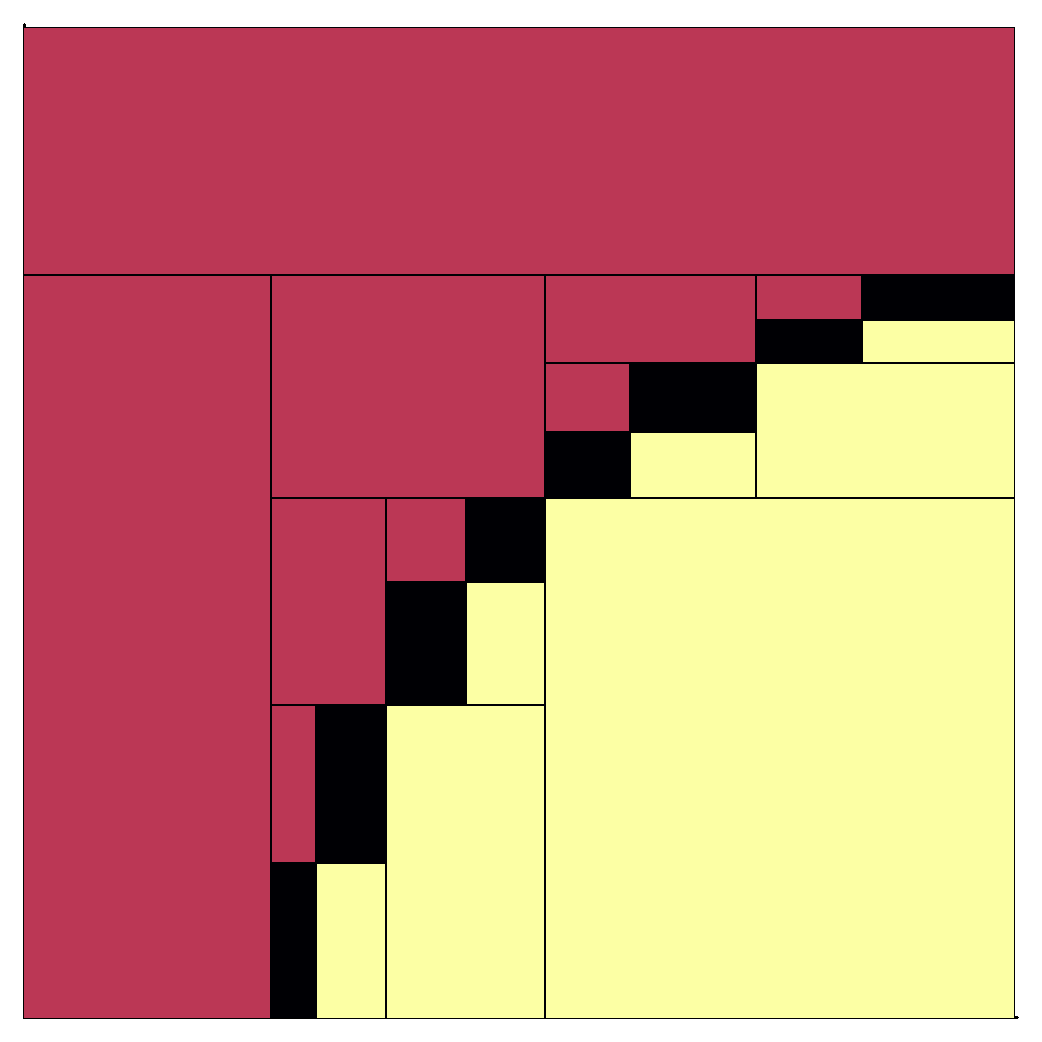
\includegraphics[width=0.23\textwidth]{./figures/nufht_boxes_lvl3.pdf}
    \hfill
    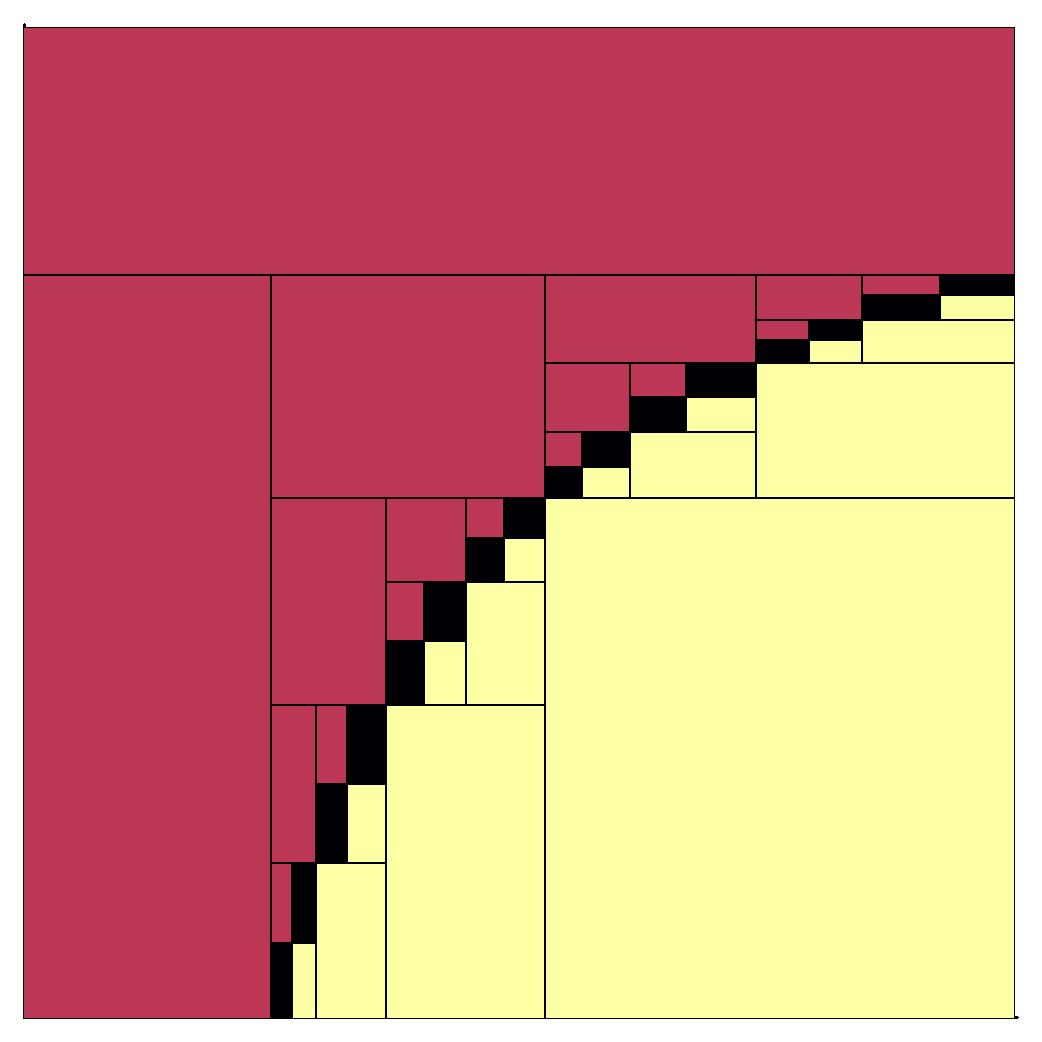
\includegraphics[width=0.23\textwidth]{./figures/nufht_boxes_lvl4.pdf}
    \caption{Direct (black), local (red), and asymptotic (yellow) boxes of
    $J_\nu(\omega_j r_k)$}
  \end{figure}

\section{Numerical experiments} \label{sec:results}
\subsection{Comparison to direct evaluation}

\subsection{Computing Fourier transforms of radial functions}

\begin{equation*}
    \hat{f}(\bm{\omega}) 
    = \int_{\R^d} f(\norm{\bm{r}}) e^{i\bm{\omega}^\top \bm{r}} d\bm{r}
    = \frac{(2\pi)^{\frac{d}{2}}}{\omega^{\frac{d}{2} - 1}} \int_0^\infty f(r) J_{\frac{d}{2} - 1}(\omega r) r^{\frac{d}{2}} dr
  \end{equation*}



\section{Discussion} \label{sec:discussion}

In this manuscript we have presented a fast algorithm for computing discrete Hankel
transforms of moderate orders from $n$ nonuniform points to $m$ nonuniform
frequencies in $\bO\big((m+n)\log\min(n,m)\big)$ operations. The algorithm
relies on a careful space-frequency analysis of the Bessel function kernel,
judicious use of small-argument series expansions and large-argument asymptotic
expansions, as well as a small number of direct calculations. The algorithm
makes no assumptions on the distribution of points in space and frequency --- it
applies to the fully nonuniform case --- and can be used for Hankel transforms
of higher order with a modest increase in computational cost. More importantly,
the algorithm does not require any precomputation, in contrast to algorithms
based on butterfly factorizations of the Hankel transform matrix. Significant
speedups over the direct calculation have been demonstrated, as well as
asymptotic scaling of the computational complexity. An implementation of the
algorithm of this paper is available as an open-source Julia package at
\href{https://github.com/pbeckman/FastHankelTransform.jl}{\texttt{github.com/pbeckman/FastHankelTransform.jl}}.

In order to efficiently extend our algorithm to compute arbitrarily high-order
Hankel transforms which are needed for higher-order Fourier-Bessel expansions
and in various high-dimensional statistical
settings~\cite{lord1954a,nolan2013multivariate}, alternative expansions and
asymptotics of~$J_\nu$ need to be used or derived. This is the focus of ongoing
research.



%%% Local Variables: % mode: latex % TeX-master: "../main" % End:


\section*{Acknowledgments}
The authors would like to thank Alex Barnett for suggesting the use of the Wimp
expansion.

\section*{Competing interests}
The authors report no competing interests.

\bibliographystyle{siamplain}
\bibliography{refs}

\end{document}

%%% Local Variables:
%%% mode: LaTeX
%%% TeX-master: t
%%% End:
